\documentclass[fr,license=none,skiptoc]{../../../eplsummary}

\usepackage{xcolor}
\usepackage{color}
\usepackage{titling}
\definecolor{violet}{RGB}{118,57,222}
\definecolor{mauvedef}{RGB}{57,0,114}
\definecolor{miorangerouge}{RGB}{215,64,0}
\newcommand{\bigO}{\ensuremath{\mathcal{O}}}

\hypertitle[es]{ définitions d'Informatique}{3}{FSAB}{1402}
{Eve Leroy}
{Peter Van Roy}

\begin{flushleft}
\renewcommand{\labelitemi}{\color{violet}{\textbullet}}
\renewcommand{\labelitemii}{\textbullet}
\renewcommand{\labelitemiii}{$\circ$}
\textcolor{mauvedef}{\underline{Abstraction de données}} : 

\begin{itemize}
\item L'intérieur est caché de l'extérieur.
\item Toutes les opérations à l'intérieur doivent passer à travers l'interface (encapsulation qui doit être supportée par le langage de programmation).
\item \underline{2 principaux types} :
\begin{itemize}[label=\textbullet]
\item \textbf{Objet} : Regroupe les valeurs et opérations en une seule entité.
\item \textbf{Type abstrait de données (ADT)} : Garde les valeurs et opérations séparées.
\end{itemize}
\end{itemize}
\begin{center}
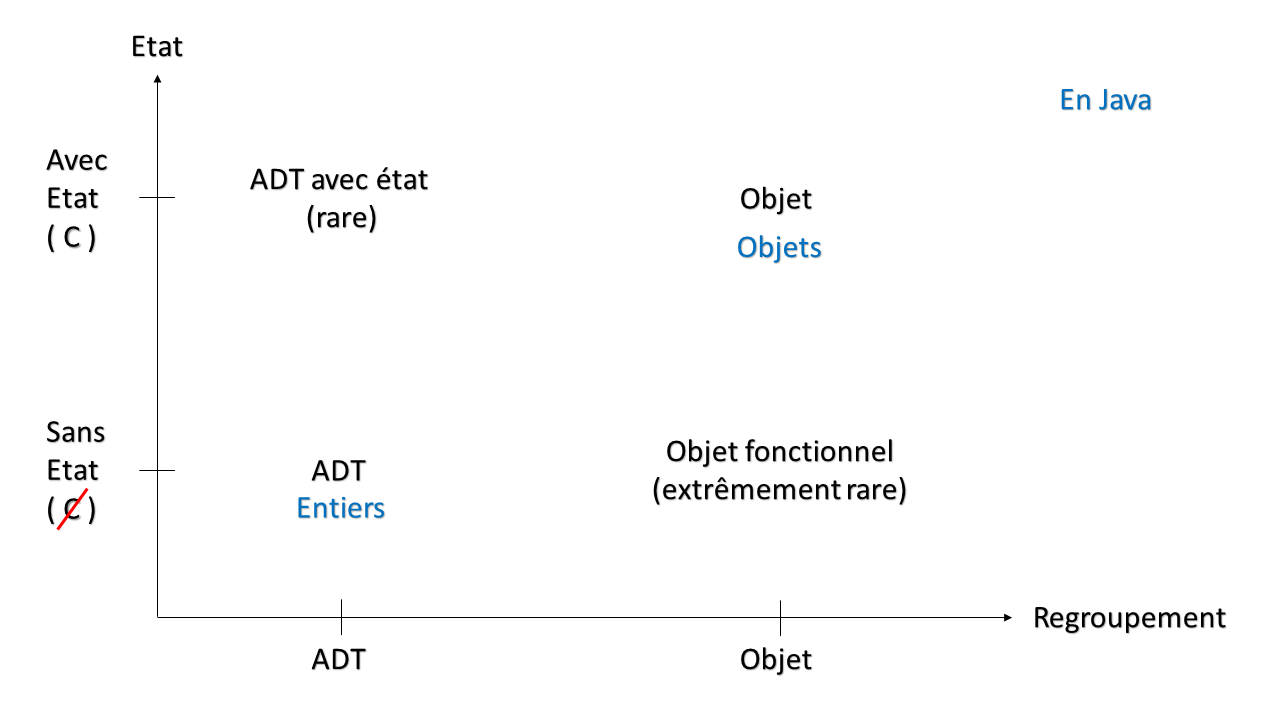
\includegraphics[scale=0.4]{ADD.png}
\label{add}
\end{center}
\bigbreak

\textcolor{mauvedef}{\underline{Abstraction procédurale}} : Toute instruction peut devenir une procédure simplement en la mettant dans une déclaration de procédure.\bigbreak

\textcolor{mauvedef}{\underline{Agent}} :

\begin{itemize}
\item Activité concurrente avec un ou plusieurs canaux de communication qui lit et écrit des flux de données.
\item Lit et réalise le flux.
\item Toute fonction qui calcule avec des listes peut être un agent.
\item La mémoire de l'agent ne grandit pas. Ceci est possible grâce aux variables à affectation unique ce qui permet donc le dataflow déterministe.
\end{itemize} \bigbreak


\textcolor{mauvedef}{\underline{Analyse asymptotique}} : 

\begin{itemize}
\item Regarder comment le temps d'exécution change quand la taille d'entrée augmente sans limite.
\item Trouver une approximation dont l'erreur tend vers 0 quand un paramètre tend vers 0.
\end{itemize} \bigbreak


\textcolor{mauvedef}{\underline{Arbre}} : Un arbre est une structure de données, de forme bifurcante et est composé soit d'une feuille (leaf), soit d'une séquence d'un élément et d'un set d'arbres.


\textcolor{blue}{$$\left\langle \text{tree T} \right\rangle ::= \text{leaf | t }(\text{T} \left\langle \text{tree T} \right\rangle   \left\langle \text{tree T} \right\rangle \ldots )$$} 


\textcolor{mauvedef}{\underline{Arbre binaire ordonné}} : 

\textcolor{blue}{$$\left\langle \text{obtree T} \right\rangle ::= \text{leaf | tree }(\text{key: T   value: V  left : } \left\langle  \text{obtree T} \right\rangle  \text{ right:} \left\langle \text{obtree T} \right\rangle )$$} 

\begin{itemize}
\item \textbf{Binaire} : Chaque arbre (non feuille) a deux sous-arbres (left \& right).
\item \textbf{Ordonné} : Pour chaque arbre et sous-arbre :

Toutes les clés du sous-arbre de gauche $<$ Clé du noeud $<$ Toutes les clés du sous-arbre de droite.
\end{itemize} \bigbreak


\textcolor{mauvedef}{\underline{Arbre de recherche}} : Arbre utilisé pour rechercher des informations, insérer des informations ou enlever des informations. \bigbreak

\textcolor{mauvedef}{\underline{Atome}} :

\begin{itemize}
\item Valeur symbolique représentée par une séquence de lettres et de chiffres. Il commence par une lettre minuscule. C'est une séquence de n'importe quels caractères délimitée par des apostrophes.
\item C'est un enregistrement dont la longueur vaut 0. Il n'a pas de noms de champs.
\end{itemize} \bigbreak


\textcolor{mauvedef}{\underline{Boucle}} : Partie d'un programme qui est répétée jusqu'à ce qu'une condition soit satisfaite. \bigbreak

\textcolor{mauvedef}{\underline{Calcul}} :

\begin{itemize}
\item Séquence d’états d’exécution qui commence par un état initial \textcolor{miorangerouge}{( [ ( $\left\langle s \right\rangle$ , $\emptyset$ ) ] , $\emptyset$ )}.
\item \textcolor{miorangerouge}{$ (ST_{0} , \sigma_{0}) \rightarrow (ST_{1} , \sigma_{1}) \rightarrow (ST_{2} , \sigma_{2})  \rightarrow   \ldots  $}
\end{itemize} \bigbreak


\textcolor{mauvedef}{\underline{Cellule}} : "Boîte" ayant un nom (identité) et un contenu. Le contenu de la boîte peut changer mais pas son identité. \bigbreak


\textcolor{mauvedef}{\underline{Classe}} : Enregistrement regroupant les attributs et les méthodes. Tous les objets créés dans une même classe ont le même comportement. Séparation entre la définition de l'objet et sa création.
	
\begin{itemize}
\item \textbf{Classe abstraite} : N'implémente pas toutes ses méthodes et ne peut donc être instanciée.
\item \textbf{Classe concrète} : Implémente toutes ses méthodes, peut hériter d’une classe abstraite, peut être instanciée.
\end{itemize}
\bigbreak


\textcolor{mauvedef}{\underline{Clause}} : Combinaison du pattern et du code qui est exécuté si le pattern est vrai. Les clauses sont indépendantes entre elles, on peut les échanger. \textit{Remarque} : Il ne faut pas oublier que dans certains cas, il y a des clauses qui sont plus globales et que du coup il faut les mettre dans l'ordre de la plus à la moins contraignante. \bigbreak


\textcolor{mauvedef}{\underline{Complexité calculatoire}} : Utilisation d'une analyse asymptotique pour étudier le temps d'exécution et l'utilisation de la mémoire des programmes (temps et espace). $f(n) =$ temps en $\mu s$ ($10^{-6} s$) pour une taille d'entrée n.
\bigbreak


\textcolor{mauvedef}{\underline{Complexité spatiale}} : C’est l'utilisation de la mémoire d’un programme en fonction de la taille de l’entrée, à un facteur constant près. Analyse asymptotique de l'espace utilisé. \textit{Remarque} : La taille augmente à l'infini et les facteurs constants sont ignorés.

\begin{itemize}
\item \underline{\textbf {Mémoire active}}

\begin{itemize}
\item Nombre total de mots utilisés par le programme au temps t.
\item $m_{active} (n,t)$ en mots de mémoire.
\end{itemize} \smallbreak

\item \underline{\textbf {Consommation de mémoire}}

\begin{itemize}
\item Nombre de mots alloués par seconde au temps t.
\item $m_{consume} (n,t)$ en mots/sec.
\end{itemize}
\item Si le programme a besoin de beaucoup (resp. peu) de données temporaires, la consommation de mémoire sera plus grande (resp. petite).

\end{itemize} \bigbreak


\textcolor{mauvedef}{\underline{Complexité temporelle}} : C’est le temps d’exécution d’un programme en fonction de la taille de l’entrée, à un facteur constant près. Analyse asymptotique du nombre d'opérations effectuées. \textit{Remarque} : La taille augmente à l'infini et les facteurs constants sont ignorés.

\begin{itemize}
\item \underline{\textbf {Les bornes}}

\begin{itemize}
\item \textbf{Notation big-$\bigO$} :
$$f(n) \in \bigO (g(n)) \text{ si } \exists C > 0, \exists n_0 \ge 1 \text{ tels que } \forall n \ge n_0 : f(n) \le C \cdot g(n)   $$
$$g(n) = \text{Limite maximale/supérieure du temps d'exécution}$$
\newpage
\item \textbf{Notation big-$\Omega$} :
$$f(n) \in \Omega (g(n)) \text{  si  } g(n) \in \bigO (f(n))$$
\begin{center} Si f est une limite supérieure à g, alors g est une limite inférieure à f. \end{center}
$$g(n) = \text{Limite minimale/inférieure du temps d'exécution}$$

\item \textbf{Notation big-$\Theta$} : Équivalence asymptotique (borne supérieure et inférieure).
$$f(n) \in \Theta (g(n)) \text{  si  } f(n) \in \bigO (g(n))  \text{  \underline{et}  } f(n) \in \Omega (g(n))$$

\end{itemize} \smallbreak

\item \underline{\textbf {La distribution des entrées}} (toujours en fonction de la taille des entrées (asymptotique))

\begin{itemize}
\item \textbf{Pire cas} : Les entrées qui ont besoin de beaucoup de calculs.
\item \textbf{Meilleur cas} : Les entrées qui peuvent être calculées facilement.
\item \textbf{Cas moyen} : Cas "typique" des entrées.
\end{itemize}

\end{itemize} \bigbreak


\textcolor{mauvedef}{\underline{Concurrence}} : Propriété de systèmes dans lesquels plusieurs opérations, calculs, sont exécutés simultanément et interagissent potentiellement entre eux.\bigbreak


\textcolor{mauvedef}{\underline{Condition d’activation}} : Condition qui doit être vraie pour que l’exécution continue. \bigbreak


\textcolor{mauvedef}{\underline{Consommateur}} : Lit le flux de données et réalise des actions. \bigbreak


\textcolor{mauvedef}{\underline{Consommation de mémoire}} : V/S mémoire active. Combien de mots sont dans l'état actif. Taux d'allocation de mémoire du programme pendant son exécution.

\underline{Ex} : Simulation de molécules bougeant dans une boîte.

\begin{itemize}
\item Grande consommation de mémoire ( = position de chaque molécule recalculée à chaque pas. Calcul difficile. Besoin de beaucoup de données temporaires).
\item Petite mémoire active ( = besoin de peu de mémoire pour garder les positions et vitesses des molécules).
\end{itemize} \bigbreak


\textcolor{mauvedef}{\underline{Cycle de vie d'un mot}} : 

\begin{center}
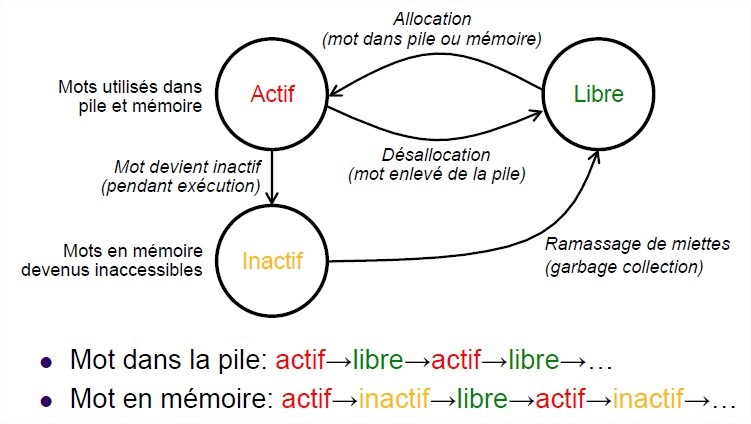
\includegraphics[scale=0.5]{CycleVie.jpg}
\end{center}


\textcolor{mauvedef}{\underline{Déterminisme}} : 
\begin{itemize}
\item Si on donne les mêmes inputs à un programme, il donnera toujours les mêmes outputs.
\item Chaque fil exécute toujours les mêmes instructions dans le même ordre.
\end{itemize}
\bigbreak

\textcolor{mauvedef}{\underline{Dictionnaire}} : Tableau dynamique où les indices sont des constantes. Ces indices sont appelés les clés (atomes, entiers, ...). \bigbreak


\textcolor{mauvedef}{\underline{Encapsulation}} : Procédé visant à empêcher la modification d'une implémentation tout en pouvant l'utiliser au moyen d'une interface. \bigbreak



\textcolor{mauvedef}{\underline{Enregistrement}} :

\begin{itemize}
\item Type général de données composées. Collection de taille fixe d’éléments accessibles par leurs noms (le nom/identificateur est soit un entier, soit un atome). Un enregistrement a une étiquette, des champs (traits) et des noms de champs. Dans le langage noyau, il n’y a que des enregistrements. \textit{Remarque} : dans un enregistrement, tous les champs sans nom sont numérotés consécutivement à partir de 1.
\item Liste $<$ Tuple $<$ Enregistrement ($x < y =$ x est plus précis que y).
\end{itemize} \bigbreak



\textcolor{mauvedef}{\underline{Environnement}} (\textcolor{miorangerouge}{E}) : Correspondance des identificateurs vers des entités dans \textcolor{miorangerouge}{$\sigma$}. L’environnement \textcolor{miorangerouge}{E} est donc l'ensemble des paires du type : identificateur $\rightarrow$ variable en mémoire.\bigbreak

\textcolor{mauvedef}{\underline{Environnement contextuel}} : L’environnement contextuel est un environnement qui fait partie de la définition d’une procédure et qui mémorise les différents identificateurs utilisés lors de la définition de la procédure. Contient les identificateurs libres. L'environnement contextuel contient tous les identifiants utilisés à l'intérieur de la fonction/procédure mais dont la définition/déclaration est réalisée à l'extérieur de cette fonction/procédure.  \bigbreak

\textcolor{mauvedef}{\underline{État}} : Séquence de valeurs calculées progressivement, qui contiennent les résultats intermédiaires d'un calcul.
\begin{itemize}
\item \textbf{État implicite} : Qui n'existe que dans l'esprit du programmeur, qui est indivisible pour le programme (\underline{Ex} : accumulateur dans le modèle déclaratif).
\item \textbf{État explicite} : Qui consiste en l'utilisation de cellules, ce qui est avantageux pour la modularité des programmes mais désavantageux pour leur exactitude (\underline{Ex} : un programme qui fonctionne aujourd'hui peut être cassé demain). Le programme peut s'observer lui-même.
\end{itemize}
\bigbreak


\textcolor{mauvedef}{\underline{État d’exécution}} \textcolor{miorangerouge}{(ST, $\sigma$)} : \textcolor{miorangerouge}{ST} = pile d’instructions sémantiques, \textcolor{miorangerouge}{$\sigma$} = mémoire.\bigbreak


\textcolor{mauvedef}{\underline{Exception}} :

\begin{itemize}
\item \textbf{En Java} : Objet héritant de la classe Exception qui est une sous-classe de Throwable.

\begin{itemize}[label=\textbullet]
\item \textbf{Checked exception} : Le compilateur vérifie que toutes les méthodes ne lancent que des exceptions déclarées pour la classe. Elles font partie de l'interface du programme.
\item \textbf{Unchecked exception} : Quelques exceptions que le compilateur ne peut pas vérifier. Héritent de RuntimeException et d'Error.
\end{itemize}

\item Nouvelles instructions :

\begin{itemize}[label=\textbullet]
\item \textbf{try} : \textcolor{miorangerouge}{try $\left\langle s \right\rangle$ catch $\left\langle x \right\rangle$ then $\left\langle s \right\rangle_1$ end } Crée un contexte de capture d'exceptions avec un traitement d'exceptions. Des instructions try imbriquées créent des contextes imbriqués.


\item \textbf{raise} : \textcolor{miorangerouge}{raise $\left\langle x \right\rangle$ end } Lève une exception. L'instruction raise fait un saut jusqu'à la frontière du contexte de capture d'exceptions le plus imbriqué et elle appelle ensuite le traitement d'exceptions de ce contexte.
\end{itemize}

\item Ce qui se passe sur la pile sémantique :
\begin{itemize}[label=\textbullet]
\item \textcolor{miorangerouge}{try $\left\langle s \right\rangle$ catch $\left\langle x \right\rangle$ then $\left\langle s \right\rangle_1$ end } $=$ \textcolor{miorangerouge}{$\left\langle s \right\rangle$} si \textcolor{miorangerouge}{$\left\langle s \right\rangle$} ne lève pas une exception.
\item Si \textcolor{miorangerouge}{$\left\langle s \right\rangle$} lève une exception, par l'exécution d'une instruction \textcolor{miorangerouge}{raise}, alors l'exécution (en cours) de \textcolor{miorangerouge}{$\left\langle s \right\rangle$} est annulée. Toutes les informations associées à \textcolor{miorangerouge}{$\left\langle s \right\rangle$} sont enlevées de la pile sémantique. Le contrôle est transféré à \textcolor{miorangerouge}{$\left\langle s \right\rangle_1$} et une référence à l'exception est donnée à \textcolor{miorangerouge}{$\left\langle x \right\rangle$}.

\end{itemize}

\item \textbf{Principe d'endiguement} : Création de contextes imbriqués avec transfert de contrôle au contexte le plus proche.

\end{itemize}

\begin{center}
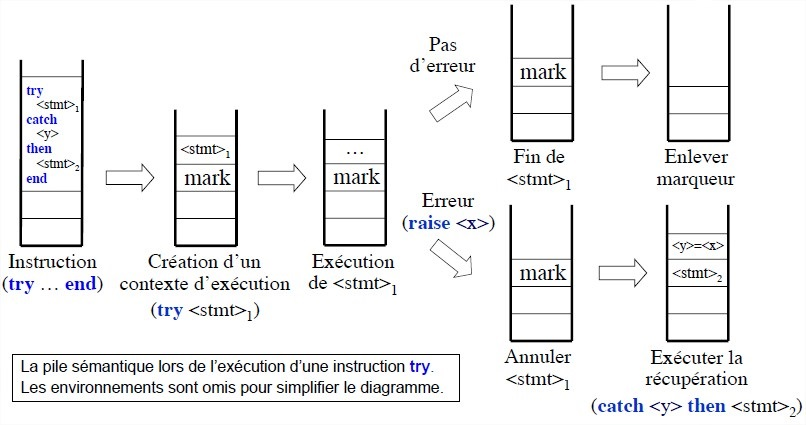
\includegraphics[scale=0.7]{Exc.jpg}
\end{center}
\bigbreak


\textcolor{mauvedef}{\underline{Fil/thread}} : Une activité est une séquence d’instructions à exécuter. Chaque fil est séquentiel et indépendant. Deux fils peuvent communiquer s'ils ont une variable en commun. Nouvelle pile sémantique créée pour chaque fil. \textit{Remarque} : Tous les fils partagent la même mémoire. 

\begin{itemize}
\item \textbf{Ordre total} : Dans un programme séquentiel, tous les pas d'exécution sont dans un ordre total. Dans un programme concurrent, tous les pas d'exécution de chaque fil sont dans un ordre total.
\item \textbf{Ordre partiel} : Les pas d'exécution de tout le programme concurrent sont dans un ordre partiel.
\item On dit que deux pas ont un \textbf{lien causal} si :
\begin{itemize}[label=\textbullet]
\item Ils sont dans le même fil.
\item Le premier lie une variable dataflow et le deuxième a besoin de la valeur de cette variable.
\item Il y a un pas intermédiaire qui a un lien de causalité avec les deux (transitivité).
\end{itemize}
\end{itemize}
\begin{center}
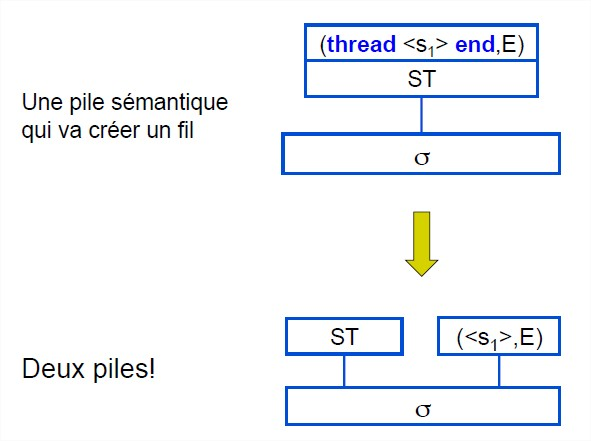
\includegraphics[scale=0.35]{PileS.jpg}
\end{center}
\bigbreak



\textcolor{mauvedef}{\underline{Flux/flot/stream}} : 
\begin{itemize}
\item Liste dont l'extrémité est une variable non liée. \underline{Ex} : $S=a|b|c|S_2$ et puis on rajoute par exemple $S_2=d|nil$
\item Un flux peut servir comme un canal de communication entre deux fils. Le premier fil ajoute des éléments au flux et le second fil lit le flux.
\end{itemize} \bigbreak





\textcolor{mauvedef}{\underline{Héritage}} : Manière de construire une classe à partir d’une autre.  En effet, il est possible de construire une abstraction de données de façon incrémentale comme une modification d’une autre abstraction de données. Il peut y avoir transformation syntaxique ou sémantique. Définition incrémentale des classes.

\begin{itemize}
\item \textbf{Lien dynamique} : \textcolor{miorangerouge}{$\{$Self M$\}$} : On sélectionne la méthode dans la classe de l’objet lui-même. Cette classe n’est connue qu’à l’exécution, c’est pourquoi il s’agit du lien dynamique.
\item \textbf{Lien fixe/statique} : \textcolor{miorangerouge}{SuperClass, M} : On sélectionne la méthode dans la super classe. Celle-ci est connue à la compilation, c’est pourquoi on l’appelle lien statique. On en a seulement besoin pour réécrire une méthode existante. Quand une méthode est réécrite, la nouvelle définition a souvent un accès à l'ancienne.
\item La composition est meilleure que l'héritage.
\item \textbf{Principe de substitution} : Supposons que A hérite de B avec les objets $O_A$ et $O_B$.
\begin{itemize}
\item Chaque procédure qui accepte $O_B$ doit accepter $O_A$.
\item Si ce principe est suivi, alors l'héritage ne casse pas et nous disons que A est une \textbf{extension conservatrice} de B.
\end{itemize}
\end{itemize} \bigbreak

\textcolor{mauvedef}{\underline{Identificateur}} : 

\begin{itemize}
\item Une chaîne de caractères dans le code source d’un programme qui fait référence pendant l’exécution à une variable en mémoire. Commence par une majuscule.
\item \textbf{Exemple} : local X in X $=2+2$ end 

X est un identificateur dans ce fragment.
\end{itemize} \bigbreak


\textcolor{mauvedef}{\underline{Identificateur libre}} :

\begin{itemize}
\item Un identificateur libre dans une instruction est un identificateur qui n’est pas défini dans cette instruction.
\item \textbf{Exemple} : local X in X $=$ Y $+$ $2$ end 

Y est un identificateur libre dans ce fragment

X n’est pas libre parce qu’il est déclaré dans ce fragment
\end{itemize} \bigbreak


\textcolor{mauvedef}{\underline{Instruction sémantique}} \textcolor{miorangerouge}{($\left\langle s \right\rangle  ,E$)} :

\begin{itemize}
\item \textcolor{miorangerouge}{$\left\langle s \right\rangle$} = instruction , \textcolor{miorangerouge}{E} = environnement.
\item Montre la relation entre une instruction et ce qu’elle référence en mémoire.
\end{itemize} \bigbreak


\textcolor{mauvedef}{\underline{Interface}} : Set d'opérations qui peuvent être utilisées selon certaines règles. Si les règles sont correctement utilisées, les résultats seront corrects (voir abstraction de données).\bigbreak


\textcolor{mauvedef}{\underline{Invariant}} : Formule mathématique exprimant la relation entre les arguments et le résultat d’une fonction, et qui est vraie à chaque appel récursif de cette fonction (pendant l'exécution). \bigbreak


\textcolor{mauvedef}{\underline{Langage noyau}} : Langage simple, basé sur un petit nombre de concepts significatifs, ayant tous les concepts essentiels. Son but est la simplicité. Toute opération du langage peut être traduite. Il est le langage par lequel tout programme va être exécuté après traduction. \bigbreak


\textcolor{mauvedef}{\underline{Liste}} :

\begin{itemize}
\item Séquence d'éléments ordonnés.
\item Type de données récursif.
\item Enregistrements nil et H|T. ( H|T = '|' (H T) = '|' (1:H  2:T) )
\textcolor{blue}{$$\left\langle \text{list} \right\rangle ::= \text{nil} \text{ } | \text{ }  \text{'|'} (1 : \left\langle \text{value} \right\rangle \text{ }  2 : \left\langle \text{list} \right\rangle )$$} 
\end{itemize}


\textcolor{mauvedef}{\underline{Loi de Moore}} :

\begin{itemize}
\item La densité ($/cm^2$) des circuits intégrés double environ tous les 2 ans.
\item Sauf pour la fréquence d'horloge qui n'augmente pas de la même façon. Plateau aujourd'hui à 3GHz. mais la densité des circuits augmente $\rightarrow$ processeurs multi-coeurs.
\end{itemize} \bigbreak


\textcolor{mauvedef}{\underline{Machine abstraite}} : Ordinateur simplifié avec une définition mathématique précise.
\begin{itemize}

\item \textbf{2 mémoires} : \textcolor{miorangerouge}{$\sigma = \sigma_1 \cup \sigma_2$}.

\begin{itemize}[label=\textbullet]
\item \textbf{Assignation unique} (variables : mémoire immuable) : \textcolor{miorangerouge}{$\sigma_1 = \{t, u, x = \xi , y = \zeta , z = 10, w = 5 \}$}

\begin{itemize}[label=$\circ$]
\item Les variables peuvent être liées ou pas.
\item Les 2 cellules sont x et y.
\item Leurs noms (constantes) respectifs sont $\xi$ et $\zeta$.
\end{itemize}

\item \textbf{Assignation multiple} (cellules (paire de 2 variables)) : \textcolor{miorangerouge}{$\sigma_2 = \{ x:t , y:w \}$}

\begin{itemize}[label=$\circ$]
\item t et w sont les contenus respectifs des deux cellules.
\end{itemize}

\item \textit{Remarque} : \textbf{Assigner un nouveau contenu à la cellule} : 

\begin{itemize}[label=$\circ$]
\item Paire changée : $2^e$ variable de la paire remplacée par une autre variable (la $1^e$ variable reste la même). \underline{Ex} : X:=Z change x:t en x:z.
\item Les variables ne changent pas ! La mémoire à assignation unique reste inchangée lorsqu'une cellule est assignée.
\end{itemize}

\end{itemize}

\item \textbf{1 environnement} \textcolor{miorangerouge}{$E = \{ X \rightarrow x, Y \rightarrow y \}$}
\item \textbf{Instruction} \textcolor{miorangerouge}{$(\left\langle s \right\rangle)$} \textbf{sémantique}  \textcolor{miorangerouge}{$(\left\langle s \right\rangle  ,E)$}
\item \textbf{Pile sémantique}  \textcolor{miorangerouge}{$ST = [(\left\langle s_1 \right\rangle  ,E_1), \ldots ,(\left\langle s_n \right\rangle  ,E_n)]$}
\item \textbf{État d’exécution} \textcolor{miorangerouge}{(ST, $\sigma$)}
\item \textbf{Exécution} \textcolor{miorangerouge}{$ (ST_{0} , \sigma_{0}) \rightarrow (ST_{1} , \sigma_{1}) \rightarrow (ST_{2} , \sigma_{2})  \rightarrow   \ldots  $}
\end{itemize} \bigbreak



\textcolor{mauvedef}{\underline{Mémoire active}} : V/S consommation de mémoire. Combien de mots/sec bougent de libre à actif. Quantité de mémoire nécessaire au programme pour continuer son exécution.

\underline{Ex} : Database en mémoire.

\begin{itemize}
\item Grande mémoire active ( = taille de la database).
\item Petite consommation de mémoire ( = besoin de peu de mémoire pour calculer le résultat d'une recherche).
\end{itemize} \bigbreak


\textcolor{mauvedef}{\underline{Mémoire à affectation unique}} (\textcolor{miorangerouge}{$\sigma$}) : Ensemble de variables pouvant être liées à une valeur :

\begin{itemize}
\item Égales mais non liées.
\item Liées à un nombre, enregistrement, procédure.
\end{itemize} \bigbreak

\textcolor{mauvedef}{\underline{Mémoïsation}} : Technique d'optimisation de code consistant à réduire le temps d'exécution d'une fonction en mémorisant ses résultats d'une fois sur l'autre. Appels de fonctions évitent le calcul des résultats précédents. \bigbreak


\textcolor{mauvedef}{\underline{Modularité}} : Un programme/système est modulaire par rapport à une partie donnée si cette partie peut être changée sans changer le reste du programme. Une partie peut être une fonction, une procédure, un composant, un module, une classe, ... \bigbreak


\textcolor{mauvedef}{\underline{Mot}} : 
\begin{itemize}
\item Ensemble de bits (chiffres binaires) dans la mémoire d’un ordinateur (pour les ordinateurs actuels un mot a une taille de 32 bits ou 64 bits).
\item Les mots sont utilisés pour représenter l’information dans la machine abstraite (pile sémantique et mémoire).
\item Un mot peut être utilisé plusieurs fois pendant l’exécution d’un programme.
\item À chaque utilisation, le mot est utilisé pour représenter une nouvelle information dans l’exécution (les mots ne se souviennent pas de leurs anciennes utilisations).
\end{itemize}
\bigbreak


\textcolor{mauvedef}{\underline{Motif de conception}} : Technique qui permet de résoudre un problème de conception (problèmes communs) et qui peut facilement être réutilisée.\bigbreak




\textcolor{mauvedef}{\underline{Non-déterminisme}} : Capacité d'un système à réaliser des décisions qui sont visibles par un programme en cours.
\begin{itemize}
\item Le programmeur ne prend pas les décisions.
\item Les décisions peuvent varier d'une exécution à une autre.
\item \textbf{Ordonnanceur} : Partie du système qui décide à quel moment utiliser quel fil (soit en choisissant le temps alloué à chaque fil soit en choisissant le nombre de calculs effectués sur chaque fil).
\item \textbf{Concurrency transparency/la concurrence pour les nuls} : Possibilité d'ajouter des fils à volonté à un programme fonctionnel sans que le résultat change. \textit{Remarque} : Attention, ne fonctionne pas pour des programmes utilisant des cellules (paradigme impératif ou orienté objet).
\end{itemize}
\bigbreak


\textcolor{mauvedef}{\underline{Objet}} : Abstraction de données qui contient la valeur et les opérations. Un objet est un ensemble de procédures visibles (les « méthodes ») qui ont accès à un état caché de cellules (les « attributs »). \bigbreak



\textcolor{mauvedef}{\underline{Occurrence d’un identificateur dans une instruction}} :

\begin{itemize}
\item Liée par rapport à une instruction \textcolor{miorangerouge}{$\left\langle s \right\rangle$} si elle est déclarée dans \textcolor{miorangerouge}{$\left\langle s \right\rangle$} (local, case, déclaration d’une procédure). Si le programme peut être exécuté.
\item \underline{Libre} : Pas lié. Existe seulement dans les instructions que l’on ne peut pas exécuter.  N’existe pas à l’exécution ($\ne$ variable liée).
\end{itemize} \bigbreak



\textcolor{mauvedef}{\underline{Ordonnanceur}} :

\begin{itemize}
\item Partie du système qui pour chaque état choisit le fil qui doit être exécuté. Il utilise un ensemble de règles précises = l’algorithme d’ordonnancement.
\item Il est équitable : Chaque fil sera exécuté.
\item Il existe des priorités entre les fils. \underline{Ex} : réseau $>$ calcul. Le programmeur a un peu de contrôle sur les priorités des fils.
\end{itemize} \bigbreak


\textcolor{mauvedef}{\underline{Ordre d'une fonction/procédure}} :

\begin{itemize}
\item \textbf{Fonction de $1^{er}$ ordre} : Fonction dont les arguments d'entrée et de sortie ne sont pas des fonctions.
\item \textbf{Fonction d'ordre N+1} : Fonction dont les arguments d'entrée et de sortie contiennent une fonction d'ordre maximum N.
\end{itemize} \bigbreak


\textcolor{mauvedef}{\underline{Paradigme}} : Approche de programmation basée sur des principes cohérents et sur de la théorie mathématique. Un paradigme est un modèle de programmation, une façon de programmer. \underline{Ex} : programmation déclarative, concurrente, avec état, orientée objet, ...\bigbreak




\textcolor{mauvedef}{\underline{Pas d’exécution}} : Chaque transition dans un calcul. \bigbreak

\textcolor{mauvedef}{\underline{Pattern matching}} : C’est la comparaison de la variable avec des formes spécifiées par le programmeur. \textit{Remarque} : la première clause qui correspond est exécutée, pas les autres. \bigbreak

\textcolor{mauvedef}{\underline{Pile (FILO : First-In Last-Out)}} : Structure de données où l’on ajoute des éléments par le début (push) et où on les enlève par le début (pop). \bigbreak


\textcolor{mauvedef}{\underline{Pile sémantique}}  (\textcolor{miorangerouge}{$ST = [(\left\langle s_1 \right\rangle  ,E_1), \ldots ,(\left\langle s_n \right\rangle  ,E_n)]$})
Une pile d'instructions sémantiques. \bigbreak

\textcolor{mauvedef}{\underline{Pipeline}} : Séquence d’objets à flux dont chacun alimente le suivant. \bigbreak


\textcolor{mauvedef}{\underline{Polymorphisme}} :
\begin{itemize}
\item Une opération est polymorphique si elle fonctionne pour des arguments de différents types. \underline{Ex} : Un message objet est polymorphique si beaucoup d'objets différents l'acceptent.
\item La même interface pour des abstractions différentes.
\item \textbf{Principe de responsabilité} : Le polymorphisme est essentiel pour répartir la responsabilité à différentes parties du programme. Une responsabilité reste concentrée à un endroit (pas splitée).
\end{itemize}\bigbreak



\textcolor{mauvedef}{\underline{Portée de l’identificateur}} : La région du programme dans laquelle un identificateur référence une variable particulière. En dehors de la portée, l’identificateur n’a pas la même référence. \bigbreak


\textcolor{mauvedef}{\underline{Portée dynamique}} :

\begin{itemize}
\item La variable qui correspond à une occurrence d’un identificateur est celle définie dans la déclaration qui contient l’occurrence et qui est la plus récente pendant l’exécution qui mène jusqu’à l’instruction qui contient l’occurrence.
\item La valeur d’une référence externe est sa valeur lors de l’appel de la procédure.
\end{itemize}\bigbreak

\textcolor{mauvedef}{\underline{Portée lexicale/statique}} :

\begin{itemize}
\item La variable qui correspond à une occurrence d’un identificateur est celle définie dans la déclaration qui contient l’occurrence et qui est la plus proche de l’occurrence dans le texte du programme.
\item La valeur d’une référence externe est sa valeur lors de la définition de la procédure.
\end{itemize}\bigbreak

\textcolor{mauvedef}{\underline{Problème NP}} :
\begin{itemize}
\item Un problème est dans la classe NP si c'est possible de vérifier une solution potentielle dans une complexité de temps polynomiale. Il est simple de vérifier une solution si on a un candidat mais trouver une solution peut être bien plus difficile. 
\item NP = Nondeterministic Polynomial time.
\end{itemize}
\bigbreak

\textcolor{mauvedef}{\underline{Problème NP-complet}} :
\begin{itemize}
\item Quelques problèmes dans NP ont comme propriété que si un algorithme efficace pour ceux-là peut être trouvé, alors c'est possible d'en dériver un algorithme efficace pour tous les problèmes NP.
\item Si on trouve un algorithme au temps polynomial pour n'importe que problème NP-complet, tous les problèmes dans NP ont des algorithmes polynomiaux.
\end{itemize}
\bigbreak



\textcolor{mauvedef}{\underline{Procédure}} : Raccourci pour un calcul (de même pour une fonction). Une procédure/fonction est une valeur en mémoire.
\begin{itemize}
\item \textbf{Appel de procédure}
\begin{itemize}
\item Crée un nouvel environnement en combinant :
\begin{itemize} [label=$\circ$]
\item L'\textcolor{miorangerouge}{$E_c$} de la procédure.
\item Les arguments formels (identifiants dans la définition de procédure). Référence les vraies valeurs des arguments.
\end{itemize}

\item Exécute le corps de procédure avec ce nouvel \textcolor{miorangerouge}{E}.
\end{itemize}



\item \textbf{Définition de procédure}
\begin{itemize}
\item Crée l'environnement contextuel.
\item Stocke la paire procédure/\textcolor{miorangerouge}{$E_c$} en mémoire, la liant à une variable (Paire instructions/environnement).
\end{itemize}



\item \textbf{Valeur de procédure}

Paire composée du corps d'une procédure et de son environnement contextuel (\textcolor{miorangerouge}{$E_{c}$}). Cette paire est gardée en mémoire et est liée à la variable qui est référée par l'identifiant qui est le nom de la procédure.
\end{itemize}\bigbreak





\textcolor{mauvedef}{\underline{Procédure anonyme}} :
\begin{itemize}
\item Procédure n'ayant pas de nom.
\item Remplacer l'identifiant par \textcolor{miorangerouge}{\$}. Il n'y a alors plus d'identifiant.
\end{itemize}\bigbreak


\textcolor{mauvedef}{\underline{Producteur}} : Génère un flux de données.  \bigbreak

\textcolor{mauvedef}{\underline{Programmation concurrente}} : Plusieurs activités en même temps. 1 thread = 1 fil = 1 pile sémantique.  \bigbreak

\textcolor{mauvedef}{\underline{Programmation déclarative}} : Dire ce que l'on veut faire, l'ordinateur trouve comment le faire.  

Une opération est déclarative si, quand on l'appelle avec les mêmes entrées, elle renvoie les mêmes résultats indépendamment de son contexte.
\begin{itemize}
\item \textbf{Indépendante} : Ne dépend pas d'un état d'exécution en dehors d'elle-même.
\item \textbf{Sans état} : N'a pas d'état d'exécution interne qui est gardé entre les appels.
\item \textbf{Déterministe} : Calcule toujours les mêmes résultats avec les mêmes entrées.
\end{itemize}\bigbreak



\textcolor{mauvedef}{\underline{Programmation fonctionnelle}} : La programmation fonctionnelle est une forme de programmation déclarative. Étant le paradigme le plus simple, elle constitue la base de tous les autres paradigmes. Dans ce modèle, un programme est une fonction ou une relation au sens mathématique.\bigbreak


\textcolor{mauvedef}{\underline{Programmation d'ordre supérieur}} : Capacité d'utiliser des fonctions (et procédure) comme des entités de première classe du langage. Elle est basée sur deux concepts : l'environnement contextuel et la valeur de procédure. \bigbreak


\textcolor{mauvedef}{\underline{Programmation orientée but}} : Généralisation de la programmation par invariants. Une propriété globale est maintenue pendant les calculs. \bigbreak


\textcolor{mauvedef}{\underline{Programmation orientée objet}} : 3 principes importants pour structurer les programmes :
\begin{itemize}
\item \textbf{Abstraction de données} : Garantie, réduit la complexité.
\item \textbf{Héritage} : Compartimentalise la responsabilité.
\item \textbf{Polymorphisme} : Évite la redondance, encourage le développement incrémental.
\end{itemize}\bigbreak


\textcolor{mauvedef}{\underline{Programmation structurée}} :
\begin{itemize}
\item Ensemble de blocs imbriqués.
\item Chaque bloc a un point d'entrée et un point de sortie.
\end{itemize}\bigbreak



\textcolor{mauvedef}{\underline{Queue (FIFO : First-In First-Out)}} : Structure de données où l’on ajoute des éléments par la fin (enqueue) et où on les enlève par le début (dequeue). \bigbreak


\textcolor{mauvedef}{\underline{Récursion}} : Fait de s'appeler soi-même. \underline{Ex} : une fonction récursive. \bigbreak


\textcolor{mauvedef}{\underline{Récursion terminale}} : L'appel récursif est la dernière opération réalisée dans le corps de la fonction. \bigbreak



\textcolor{mauvedef}{\underline{Règle de sémantique pour la composition séquentielle}} : \textcolor{miorangerouge}{$( \left\langle s_1 \right\rangle \left\langle s_2 \right\rangle )$}

\begin{itemize}
\item État d'entrée : \textcolor{miorangerouge}{$([(S_a, S_b), S_2, \ldots , S_n ], \sigma )$} 1 instruction, 2 parties
\item État de sortie : \textcolor{miorangerouge}{$([S_a, S_b, S_2, \ldots , S_n ], \sigma )$} 2 instructions

L'instruction enlève le haut de la pile et ajoute 2 nouveaux éléments.
\end{itemize}\bigbreak

\begin{center}
\begin{tabular}{|c|c|c|}
 & & $S_a$ \\
\hline
$S_a$ $S_b$ & & $S_b$\\
\hline
$S_2$ & & $S_2$\\
\hline
$\ldots$ & $\Rightarrow$ & $\ldots$\\
\hline
$S_n$ & & $S_n$\\
\hline
\end{tabular}
\end{center}
\newpage




\textcolor{mauvedef}{\underline{Règle de sémantique pour le local}} : (\textcolor{miorangerouge}{local $\left\langle x \right\rangle \text{ in } \left\langle s \right\rangle$ end})

\begin{itemize}
\item Crée une nouvelle variable \textcolor{miorangerouge}{x} en mémoire \textcolor{miorangerouge}{$\sigma$}.
\item Ajoute le lien \textcolor{miorangerouge}{$\{ X \rightarrow x \}$} à l'environnement \textcolor{miorangerouge}{E} (adjonction).
\end{itemize}\bigbreak

\begin{center}
\begin{tabular}{|c|c|c|}
(local $\left\langle x \right\rangle \text{ in } \left\langle s \right\rangle$ end, E) & & ($\left\langle s \right\rangle$, E $+ \{ \left\langle x \right\rangle \rightarrow x \}$)\\
\hline
$S_2$ & & $S_2$\\
\hline
$\ldots$ & $\Rightarrow$ & $\ldots$\\
\hline
$S_n$ & & $S_n$\\
\hline
\end{tabular}
\end{center}
\bigbreak

\begin{center}
\begin{tabular}{ccccccc}
 & & & & $\sigma$ & $\Rightarrow$ & $\sigma \cup \{x\}$\\
\end{tabular}
\end{center}
\bigbreak




\textcolor{mauvedef}{\underline{Règle de sémantique pour la procédure}} : 

\begin{itemize}
\item \textbf{Définition} : Création d'une nouvelle valeur procédurale (avec \textcolor{miorangerouge}{$E_c$}).
\item \textcolor{miorangerouge}{$\left\langle x \right\rangle_1 \ldots \left\langle x \right\rangle_n$} sont les identificateurs libres de \textcolor{miorangerouge}{$\left\langle s \right\rangle$}.
\item \textcolor{miorangerouge}{$\left\langle y \right\rangle_1 \ldots \left\langle y \right\rangle_n$} sont les arguments formels de la procédure.
\end{itemize}\bigbreak

\begin{center}
\begin{tabular}{|c|c|c|}
($\left\langle x \right\rangle = \text{ proc } \{\$ \left\langle y \right\rangle_1 \ldots \left\langle y \right\rangle_n \} \left\langle s \right\rangle$ end, E) & & \\
\hline
$S_2$ & & $S_2$\\
\hline
$\ldots$ & $\Rightarrow$ & $\ldots$\\
\hline
$S_n$ & & $S_n$\\
\hline
\end{tabular}
\end{center}
\bigbreak

\begin{center}
\begin{tabular}{ccccccc}
& & & & $E ( \left\langle x \right\rangle ) = x$ & $\Rightarrow$ & $E_c = E|_{\left\langle x \right\rangle_1 \ldots \left\langle x \right\rangle_n}$\\
 & & & & & & \\
 & & & & $\sigma = \{ x, \ldots \}$ & $\Rightarrow$ & $\sigma = \{ x = ( \text{ proc } \{ \$ \left\langle y \right\rangle_1 \ldots \left\langle y \right\rangle_n \} \left\langle s \right\rangle \text{ end}, E_c ), \ldots \}$\\
\end{tabular}
\end{center}
\bigbreak





\textcolor{mauvedef}{\underline{Règle de sémantique pour skip}} :

\begin{itemize}
\item État d'entrée : \textcolor{miorangerouge}{$([(\text{skip, E}), S_2, \ldots , S_n ], \sigma )$}
\item État de sortie : \textcolor{miorangerouge}{$([S_2, \ldots , S_n ], \sigma )$}

On enlève l'instruction et on retourne la pile sémantique.
\end{itemize}\bigbreak

\begin{center}
\begin{tabular}{|c|c|c|}
(skip, E) & & \\
\hline
$S_2$ & & $S_2$\\
\hline
$\ldots$ & $\Rightarrow$ & $\ldots$\\
\hline
$S_n$ & & $S_n$\\
\hline
\end{tabular}
\end{center}
\bigbreak



\textcolor{mauvedef}{\underline{Sémantique}} :
\begin{itemize}
\item Sémantique = sémantique formelle = sémantique mathématique.
\item Modèle mathématique précis de comment le programme s'exécute.
\item Peut être utilisé pour raisonner à propos du design et de l'exactitude du programme.
\item La sémantique comporte 2 parties :
\begin{itemize}
\item Le langage noyau (Traduction d'un langage compliqué en langage noyau).
\item La machine abstraite (Elle exécute le langage noyau).
\end{itemize}
\end{itemize}\bigbreak

\textcolor{mauvedef}{\underline{Sémantique axiomatique}} : Explique un programme comme une implication. Si certaines propriétés tiennent avant l'exécution, alors d'autres propriétés tiendront après l'exécution. \bigbreak

\textcolor{mauvedef}{\underline{Sémantique dénotationnelle}} : Explique un programme comme une fonction sur un domaine abstrait. Simplifie quelques types d'analyses mathématiques du programme. \bigbreak

\textcolor{mauvedef}{\underline{Sémantique d'entrelacement}} : L'exécution de tous les fils est entrelacée pour former une exécution globale. Chaque fil fait un petit bout à la fois. \bigbreak


\textcolor{mauvedef}{\underline{Sémantique logique}} :

\begin{itemize}
\item Explique un programme comme un modèle logique d'un set d'axiomes logiques.
\item Exécution du programme = déduction.
\item Le résultat d'un programme est une vraie propriété dérivée des axiomes.
\end{itemize}\bigbreak


\textcolor{mauvedef}{\underline{Sémantique opérationnelle}} : Sémantique qui définit le sens du langage noyau à travers son exécution sur une machine abstraite. Explique un programme en terme de son exécution sur une machine abstraite définie rigoureusement. \bigbreak


\textcolor{mauvedef}{\underline{Spécification}} :

\begin{itemize}
\item Formulation mathématique de ce que fait la fonction.
\item Définition mathématique du résultat du programme comme une fonction de l'input.
\item Besoin de prouver que le programme satisfait la spécification selon la sémantique.
\item Spécification (mathématiques/ce que l'on veut) $\underset{\text{Sémantique (lien)}}{\longleftrightarrow}$ Programme (langage de programmation/ce que l'on a)

Ce que l'on a s'exécute selon ce que l'on veut.
\end{itemize}\bigbreak


\textcolor{mauvedef}{\underline{Système multi-agent}} : 
\begin{itemize}
\item Poducteur/consommateur ou pipeline.
\item Chaque agent est une activité.
\item Les activités communiquent entre elles grâce aux canaux de communication.
\end{itemize}\bigbreak



\textcolor{mauvedef}{\underline{Transformateur}} : Fil qui lit le flux venant du producteur et crée un nouveau flux qu’il envoie aux consommateurs. \bigbreak


\textcolor{mauvedef}{\underline{Tuple}} : 

\begin{itemize}
\item C'est un enregistrement dont les noms de champs sont des entiers successifs (départ=1).
\item Si la condition est fausse, alors c'est toujours un enregistrement mais plus un tuple.
\item S'il n'y a pas de noms de champs, ils sont numérotés automatiquement en partant de 1.
\end{itemize}

\begin{center}
\textcolor{blue}{$\left\langle \text{tuple} \right\rangle ::=  \text{label }  ( \left\langle v \right\rangle_1  \left\langle v \right\rangle_2 \ldots ) $}
\end{center}

\bigbreak


\textcolor{mauvedef}{\underline{Type abstrait}} :

\begin{itemize}
\item On dit d'un type qu'il est abstrait s'il est complètement défini par l'ensemble de ses opérations, indépendamment de son implémentation.
\item $=$ ADT $=$ Manière abstraite d'utiliser des données sans dépendre d'une implémentation particulière, elle se compose d'un ensemble d'instances appelé son interface.
\end{itemize}\bigbreak




\end{flushleft}
\end{document}
%5 fixe la hauteur de l'entête
%6 fixe la distance entre l'entête et le texte
%7 fixe la hauteur du pied de page
%8 fixe la distance entre le texte et le pied de page

\title{Définitions Q3 Info}
\author{Leroy Eve}
\date{Décembre 2015}

\begin{document}

\maketitle
\begin{flushleft}


\textcolor{mauvedef}{\underline{Abstraction de données}} : 

\begin{itemize}
\item L'intérieur est caché de l'extérieur.
\item Toutes les opérations à l'intérieur doivent passer à travers l'interface (encapsulation qui doit être supportée par le langage de programmation).
\item \underline{2 principaux types} :
\begin{itemize}[label=\textbullet]
\item \textbf{Objet} : Regroupe les valeurs et opérations en une seule entité.
\item \textbf{Type abstrait de données (ADT)} : Garde les valeurs et opérations séparées.
\end{itemize}
\end{itemize}
\begin{center}
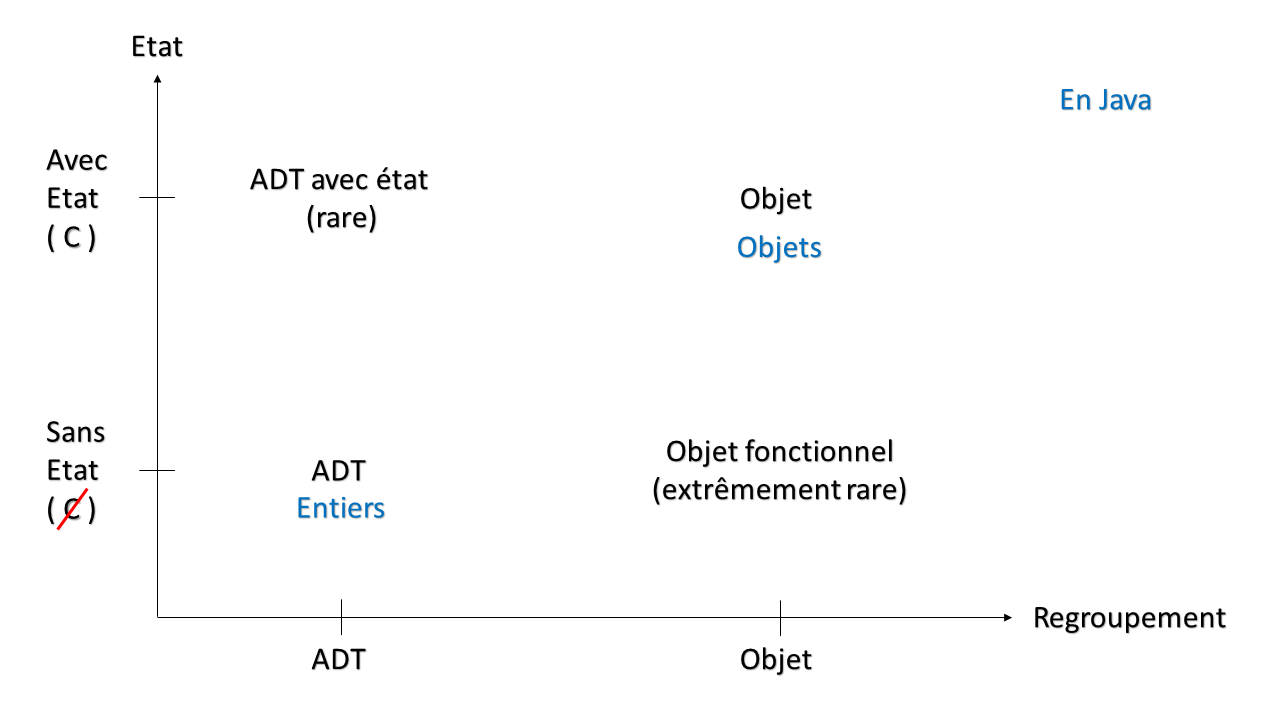
\includegraphics[scale=0.4]{ADD.png}
\label{add2}
\end{center}
\bigbreak


\textcolor{mauvedef}{\underline{Abstraction procédurale}} : Toute instruction peut devenir une procédure simplement en la mettant dans une déclaration de procédure.\bigbreak

\textcolor{mauvedef}{\underline{Agent}} :

\begin{itemize}
\item Activité concurrente avec un ou plusieurs canaux de communication qui lit et écrit des flux de données.
\item Lit et réalise le flux.
\item Toute fonction qui calcule avec des listes peut être un agent.
\item La mémoire de l'agent ne grandit pas. Ceci est possible grâce aux variables à affectation unique ce qui permet donc le dataflow déterministe.
\end{itemize} \bigbreak


\textcolor{mauvedef}{\underline{Analyse asymptotique}} : 

\begin{itemize}
\item Regarder comment le temps d'exécution change quand la taille d'entrée augmente sans limite.
\item Trouver une approximation dont l'erreur tend vers 0 quand un paramètre tend vers 0.
\end{itemize} \bigbreak


\textcolor{mauvedef}{\underline{Arbre}} : Un arbre est une structure de données, de forme bifurcante et est composé soit d'une feuille (leaf), soit d'une séquence d'un élément et d'un set d'arbres.


\textcolor{blue}{$$\left\langle \text{tree T} \right\rangle ::= \text{leaf | t }(\text{T} \left\langle \text{tree T} \right\rangle   \left\langle \text{tree T} \right\rangle \ldots )$$} 


\textcolor{mauvedef}{\underline{Arbre binaire ordonné}} : 

\textcolor{blue}{$$\left\langle \text{obtree T} \right\rangle ::= \text{leaf | tree }(\text{key: T   value: V  left : } \left\langle  \text{obtree T} \right\rangle  \text{ right:} \left\langle \text{obtree T} \right\rangle )$$} 

\begin{itemize}
\item \textbf{Binaire} : Chaque arbre (non feuille) a deux sous-arbres (left \& right).
\item \textbf{Ordonné} : Pour chaque arbre et sous-arbre :

Toutes les clés du sous-arbre de gauche $<$ Clé du noeud $<$ Toutes les clés du sous-arbre de droite.
\end{itemize} \bigbreak


\textcolor{mauvedef}{\underline{Arbre de recherche}} : Arbre utilisé pour rechercher des informations, insérer des informations ou enlever des informations. \bigbreak

\textcolor{mauvedef}{\underline{Atome}} :

\begin{itemize}
\item Valeur symbolique représentée par une séquence de lettres et de chiffres. Il commence par une lettre minuscule. C'est une séquence de n'importe quels caractères délimitée par des apostrophes.
\item C'est un enregistrement dont la longueur vaut 0. Il n'a pas de noms de champs.
\end{itemize} \bigbreak


\textcolor{mauvedef}{\underline{Boucle}} : Partie d'un programme qui est répétée jusqu'à ce qu'une condition soit satisfaite. \bigbreak

\textcolor{mauvedef}{\underline{Calcul}} :

\begin{itemize}
\item Séquence d’états d’exécution qui commence par un état initial \textcolor{miorangerouge}{( [ ( $\left\langle s \right\rangle$ , $\emptyset$ ) ] , $\emptyset$ )}.
\item \textcolor{miorangerouge}{$ (ST_{0} , \sigma_{0}) \rightarrow (ST_{1} , \sigma_{1}) \rightarrow (ST_{2} , \sigma_{2})  \rightarrow   \ldots  $}
\end{itemize} \bigbreak


\textcolor{mauvedef}{\underline{Cellule}} : "Boîte" ayant un nom (identité) et un contenu. Le contenu de la boîte peut changer mais pas son identité. \bigbreak


\textcolor{mauvedef}{\underline{Classe}} : Enregistrement regroupant les attributs et les méthodes. Tous les objets créés dans une même classe ont le même comportement. Séparation entre la définition de l'objet et sa création.
	
\begin{itemize}
\item \textbf{Classe abstraite} : N'implémente pas toutes ses méthodes et ne peut donc être instanciée.
\item \textbf{Classe concrète} : Implémente toutes ses méthodes, peut hériter d’une classe abstraite, peut être instanciée.
\end{itemize}
\bigbreak


\textcolor{mauvedef}{\underline{Clause}} : Combinaison du pattern et du code qui est exécuté si le pattern est vrai. Les clauses sont indépendantes entre elles, on peut les échanger. \textit{Remarque} : Il ne faut pas oublier que dans certains cas, il y a des clauses qui sont plus globales et que du coup il faut les mettre dans l'ordre de la plus à la moins contraignante. \bigbreak


\textcolor{mauvedef}{\underline{Complexité calculatoire}} : Utilisation d'une analyse asymptotique pour étudier le temps d'exécution et l'utilisation de la mémoire des programmes (temps et espace). $f(n) =$ temps en $\mu s$ ($10^{-6} s$) pour une taille d'entrée n.
\bigbreak


\textcolor{mauvedef}{\underline{Complexité spatiale}} : C’est l'utilisation de la mémoire d’un programme en fonction de la taille de l’entrée, à un facteur constant près. Analyse asymptotique de l'espace utilisé. \textit{Remarque} : La taille augmente à l'infini et les facteurs constants sont ignorés.

\begin{itemize}
\item \underline{\textbf {Mémoire active}}

\begin{itemize} [label=\textbullet, font=\MEDIUM]
\item Nombre total de mots utilisés par le programme au temps t.
\item $m_{active} (n,t)$ en mots de mémoire.
\end{itemize} \smallbreak

\item \underline{\textbf {Consommation de mémoire}}

\begin{itemize} [label=\textbullet, font=\MEDIUM]
\item Nombre de mots alloués par seconde au temps t.
\item $m_{consume} (n,t)$ en mots/sec.
\end{itemize}

\item Si le programme a besoin de beaucoup (resp. peu) de données temporaires, la consommation de mémoire sera plus grande (resp. petite).

\end{itemize} \bigbreak


\textcolor{mauvedef}{\underline{Complexité temporelle}} : C’est le temps d’exécution d’un programme en fonction de la taille de l’entrée, à un facteur constant près. Analyse asymptotique du nombre d'opérations effectuées. \textit{Remarque} : La taille augmente à l'infini et les facteurs constants sont ignorés.

\begin{itemize}
\item \underline{\textbf {Les bornes}}

\begin{itemize} [label=\textbullet, font=\MEDIUM]
\item \textbf{Notation big-$\bigO$} :
$$f(n) \in \bigO (g(n)) \text{ si } \exists C > 0, \exists n_0 \ge 1 \text{ tels que } \forall n \ge n_0 : f(n) \le C \cdot g(n)   $$
$$g(n) = \text{Limite maximale/supérieure du temps d'exécution}$$
\newpage
\item \textbf{Notation big-$\Omega$} :
$$f(n) \in \Omega (g(n)) \text{  si  } g(n) \in \bigO (f(n))$$
\begin{center} Si f est une limite supérieure à g, alors g est une limite inférieure à f. \end{center}
$$g(n) = \text{Limite minimale/inférieure du temps d'exécution}$$

\item \textbf{Notation big-$\Theta$} : Équivalence asymptotique (borne supérieure et inférieure).
$$f(n) \in \Theta (g(n)) \text{  si  } f(n) \in \bigO (g(n))  \text{  \underline{et}  } f(n) \in \Omega (g(n))$$


\end{itemize} \smallbreak

\item \underline{\textbf {La distribution des entrées}} (toujours en fonction de la taille des entrées (asymptotique))


\begin{itemize} [label=\textbullet, font=\MEDIUM]
\item \textbf{Pire cas} : Les entrées qui ont besoin de beaucoup de calculs.
\item \textbf{Meilleur cas} : Les entrées qui peuvent être calculées facilement.
\item \textbf{Cas moyen} : Cas "typique" des entrées.
\end{itemize}

\end{itemize} \bigbreak


\textcolor{mauvedef}{\underline{Concurrence}} : Propriété de systèmes dans lesquels plusieurs opérations, calculs, sont exécutés simultanément et interagissent potentiellement entre eux.\bigbreak


\textcolor{mauvedef}{\underline{Condition d’activation}} : Condition qui doit être vraie pour que l’exécution continue. \bigbreak


\textcolor{mauvedef}{\underline{Consommateur}} : Lit le flux de données et réalise des actions. \bigbreak


\textcolor{mauvedef}{\underline{Consommation de mémoire}} : V/S mémoire active. Combien de mots sont dans l'état actif. Taux d'allocation de mémoire du programme pendant son exécution.

\underline{Ex} : Simulation de molécules bougeant dans une boîte.

\begin{itemize}
\item Grande consommation de mémoire ( = position de chaque molécule recalculée à chaque pas. Calcul difficile. Besoin de beaucoup de données temporaires).
\item Petite mémoire active ( = besoin de peu de mémoire pour garder les positions et vitesses des molécules).
\end{itemize} \bigbreak


\textcolor{mauvedef}{\underline{Cycle de vie d'un mot}} : 

\begin{center}
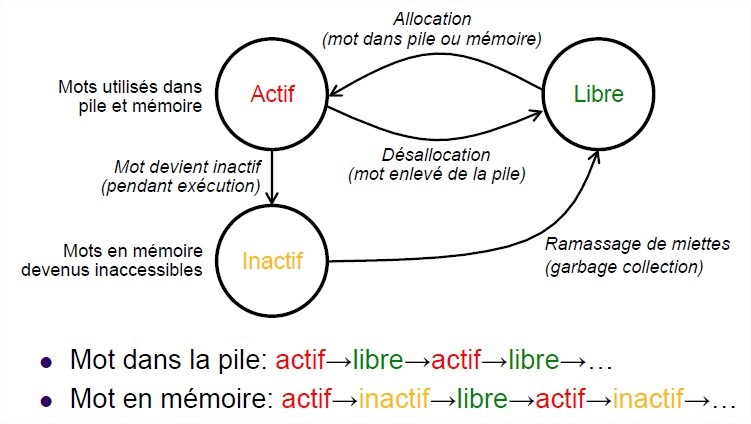
\includegraphics[scale=0.5]{CycleVie.jpg}
\end{center}


\textcolor{mauvedef}{\underline{Déterminisme}} : 
\begin{itemize}
\item Si on donne les mêmes inputs à un programme, il donnera toujours les mêmes outputs.
\item Chaque fil exécute toujours les mêmes instructions dans le même ordre.
\end{itemize}
\bigbreak

\textcolor{mauvedef}{\underline{Dictionnaire}} : Tableau dynamique où les indices sont des constantes. Ces indices sont appelés les clés (atomes, entiers, ...). \bigbreak


\textcolor{mauvedef}{\underline{Encapsulation}} : Procédé visant à empêcher la modification d'une implémentation tout en pouvant l'utiliser au moyen d'une interface. \bigbreak



\textcolor{mauvedef}{\underline{Enregistrement}} :

\begin{itemize}
\item Type général de données composées. Collection de taille fixe d’éléments accessibles par leurs noms (le nom/identificateur est soit un entier, soit un atome). Un enregistrement a une étiquette, des champs (traits) et des noms de champs. Dans le langage noyau, il n’y a que des enregistrements. \textit{Remarque} : dans un enregistrement, tous les champs sans nom sont numérotés consécutivement à partir de 1.
\item Liste $<$ Tuple $<$ Enregistrement ($x < y =$ x est plus précis que y).
\end{itemize} \bigbreak



\textcolor{mauvedef}{\underline{Environnement}} (\textcolor{miorangerouge}{E}) : Correspondance des identificateurs vers des entités dans \textcolor{miorangerouge}{$\sigma$}. L’environnement \textcolor{miorangerouge}{E} est donc l'ensemble des paires du type : identificateur $\rightarrow$ variable en mémoire.\bigbreak

\textcolor{mauvedef}{\underline{Environnement contextuel}} : L’environnement contextuel est un environnement qui fait partie de la définition d’une procédure et qui mémorise les différents identificateurs utilisés lors de la définition de la procédure. Contient les identificateurs libres. L'environnement contextuel contient tous les identifiants utilisés à l'intérieur de la fonction/procédure mais dont la définition/déclaration est réalisée à l'extérieur de cette fonction/procédure.  \bigbreak

\textcolor{mauvedef}{\underline{État}} : Séquence de valeurs calculées progressivement, qui contiennent les résultats intermédiaires d'un calcul.
\begin{itemize}
\item \textbf{État implicite} : Qui n'existe que dans l'esprit du programmeur, qui est indivisible pour le programme (\underline{Ex} : accumulateur dans le modèle déclaratif).
\item \textbf{État explicite} : Qui consiste en l'utilisation de cellules, ce qui est avantageux pour la modularité des programmes mais désavantageux pour leur exactitude (\underline{Ex} : un programme qui fonctionne aujourd'hui peut être cassé demain). Le programme peut s'observer lui-même.
\end{itemize}
\bigbreak


\textcolor{mauvedef}{\underline{État d’exécution}} \textcolor{miorangerouge}{(ST, $\sigma$)} : \textcolor{miorangerouge}{ST} = pile d’instructions sémantiques, \textcolor{miorangerouge}{$\sigma$} = mémoire.\bigbreak


\textcolor{mauvedef}{\underline{Exception}} :

\begin{itemize}
\item \textbf{En Java} : Objet héritant de la classe Exception qui est une sous-classe de Throwable.

\begin{itemize}[label=\textbullet]
\item \textbf{Checked exception} : Le compilateur vérifie que toutes les méthodes ne lancent que des exceptions déclarées pour la classe. Elles font partie de l'interface du programme.
\item \textbf{Unchecked exception} : Quelques exceptions que le compilateur ne peut pas vérifier. Héritent de RuntimeException et d'Error.
\end{itemize}

\item Nouvelles instructions :

\begin{itemize}[label=\textbullet]
\item \textbf{try} : \textcolor{miorangerouge}{try $\left\langle s \right\rangle$ catch $\left\langle x \right\rangle$ then $\left\langle s \right\rangle_1$ end } Crée un contexte de capture d'exceptions avec un traitement d'exceptions. Des instructions try imbriquées créent des contextes imbriqués.


\item \textbf{raise} : \textcolor{miorangerouge}{raise $\left\langle x \right\rangle$ end } Lève une exception. L'instruction raise fait un saut jusqu'à la frontière du contexte de capture d'exceptions le plus imbriqué et elle appelle ensuite le traitement d'exceptions de ce contexte.
\end{itemize}

\item Ce qui se passe sur la pile sémantique :
\begin{itemize}[label=\textbullet]
\item \textcolor{miorangerouge}{try $\left\langle s \right\rangle$ catch $\left\langle x \right\rangle$ then $\left\langle s \right\rangle_1$ end } $=$ \textcolor{miorangerouge}{$\left\langle s \right\rangle$} si \textcolor{miorangerouge}{$\left\langle s \right\rangle$} ne lève pas une exception.
\item Si \textcolor{miorangerouge}{$\left\langle s \right\rangle$} lève une exception, par l'exécution d'une instruction \textcolor{miorangerouge}{raise}, alors l'exécution (en cours) de \textcolor{miorangerouge}{$\left\langle s \right\rangle$} est annulée. Toutes les informations associées à \textcolor{miorangerouge}{$\left\langle s \right\rangle$} sont enlevées de la pile sémantique. Le contrôle est transféré à \textcolor{miorangerouge}{$\left\langle s \right\rangle_1$} et une référence à l'exception est donnée à \textcolor{miorangerouge}{$\left\langle x \right\rangle$}.

\end{itemize}

\item \textbf{Principe d'endiguement} : Création de contextes imbriqués avec transfert de contrôle au contexte le plus proche.

\end{itemize}

\begin{center}
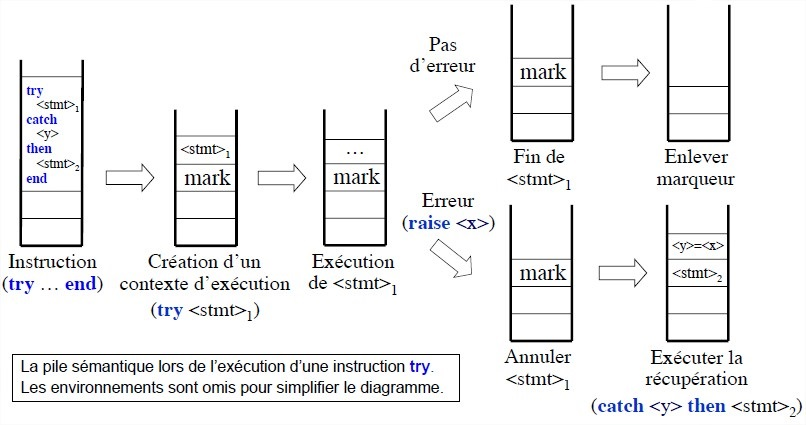
\includegraphics[scale=0.7]{Exc.jpg}
\end{center}
\bigbreak


\textcolor{mauvedef}{\underline{Fil/thread}} : Une activité est une séquence d’instructions à exécuter. Chaque fil est séquentiel et indépendant. Deux fils peuvent communiquer s'ils ont une variable en commun. Nouvelle pile sémantique créée pour chaque fil. \textit{Remarque} : Tous les fils partagent la même mémoire. 

\begin{itemize}
\item \textbf{Ordre total} : Dans un programme séquentiel, tous les pas d'exécution sont dans un ordre total. Dans un programme concurrent, tous les pas d'exécution de chaque fil sont dans un ordre total.
\item \textbf{Ordre partiel} : Les pas d'exécution de tout le programme concurrent sont dans un ordre partiel.
\item On dit que deux pas ont un \textbf{lien causal} si :
\begin{itemize}[label=\textbullet]
\item Ils sont dans le même fil.
\item Le premier lie une variable dataflow et le deuxième a besoin de la valeur de cette variable.
\item Il y a un pas intermédiaire qui a un lien de causalité avec les deux (transitivité).
\end{itemize}
\end{itemize}
\begin{center}
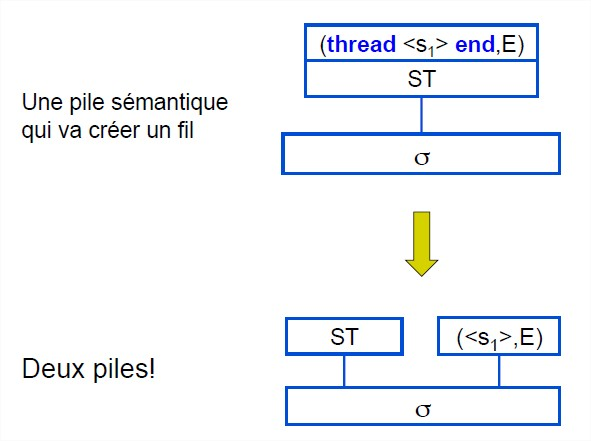
\includegraphics[scale=0.35]{PileS.jpg}
\end{center}
\bigbreak



\textcolor{mauvedef}{\underline{Flux/flot/stream}} : 
\begin{itemize}
\item Liste dont l'extrémité est une variable non liée. \underline{Ex} : $S=a|b|c|S_2$ et puis on rajoute par exemple $S_2=d|nil$
\item Un flux peut servir comme un canal de communication entre deux fils. Le premier fil ajoute des éléments au flux et le second fil lit le flux.
\end{itemize} \bigbreak





\textcolor{mauvedef}{\underline{Héritage}} : Manière de construire une classe à partir d’une autre.  En effet, il est possible de construire une abstraction de données de façon incrémentale comme une modification d’une autre abstraction de données. Il peut y avoir transformation syntaxique ou sémantique. Définition incrémentale des classes.

\begin{itemize}
\item \textbf{Lien dynamique} : \textcolor{miorangerouge}{$\{$Self M$\}$} : On sélectionne la méthode dans la classe de l’objet lui-même. Cette classe n’est connue qu’à l’exécution, c’est pourquoi il s’agit du lien dynamique.
\item \textbf{Lien fixe/statique} : \textcolor{miorangerouge}{SuperClass, M} : On sélectionne la méthode dans la super classe. Celle-ci est connue à la compilation, c’est pourquoi on l’appelle lien statique. On en a seulement besoin pour réécrire une méthode existante. Quand une méthode est réécrite, la nouvelle définition a souvent un accès à l'ancienne.
\item La composition est meilleure que l'héritage.
\item \textbf{Principe de substitution} : Supposons que A hérite de B avec les objets $O_A$ et $O_B$.
\begin{itemize}[label=\circ]
\item Chaque procédure qui accepte $O_B$ doit accepter $O_A$.
\item Si ce principe est suivi, alors l'héritage ne casse pas et nous disons que A est une \textbf{extension conservatrice} de B.
\end{itemize}
\end{itemize} \bigbreak



\textcolor{mauvedef}{\underline{Identificateur}} : 

\begin{itemize}
\item Une chaîne de caractères dans le code source d’un programme qui fait référence pendant l’exécution à une variable en mémoire. Commence par une majuscule.
\item \textbf{Exemple} : local X in X $=2+2$ end 

X est un identificateur dans ce fragment.
\end{itemize} \bigbreak


\textcolor{mauvedef}{\underline{Identificateur libre}} :

\begin{itemize}
\item Un identificateur libre dans une instruction est un identificateur qui n’est pas défini dans cette instruction.
\item \textbf{Exemple} : local X in X $=$ Y $+$ $2$ end 

Y est un identificateur libre dans ce fragment

X n’est pas libre parce qu’il est déclaré dans ce fragment
\end{itemize} \bigbreak


\textcolor{mauvedef}{\underline{Instruction sémantique}} \textcolor{miorangerouge}{($\left\langle s \right\rangle  ,E$)}} :

\begin{itemize}
\item \textcolor{miorangerouge}{$\left\langle s \right\rangle$} = instruction , \textcolor{miorangerouge}{E} = environnement.
\item Montre la relation entre une instruction et ce qu’elle référence en mémoire.
\end{itemize} \bigbreak


\textcolor{mauvedef}{\underline{Interface}} : Set d'opérations qui peuvent être utilisées selon certaines règles. Si les règles sont correctement utilisées, les résultats seront corrects (voir abstraction de données).\bigbreak


\textcolor{mauvedef}{\underline{Invariant}} : Formule mathématique exprimant la relation entre les arguments et le résultat d’une fonction, et qui est vraie à chaque appel récursif de cette fonction (pendant l'exécution). \bigbreak


\textcolor{mauvedef}{\underline{Langage noyau}} : Langage simple, basé sur un petit nombre de concepts significatifs, ayant tous les concepts essentiels. Son but est la simplicité. Toute opération du langage peut être traduite. Il est le langage par lequel tout programme va être exécuté après traduction. \bigbreak


\textcolor{mauvedef}{\underline{Liste}} :

\begin{itemize}
\item Séquence d'éléments ordonnés.
\item Type de données récursif.
\item Enregistrements nil et H|T. ( H|T = '|' (H T) = '|' (1:H  2:T) )
\textcolor{blue}{$$\left\langle \text{list} \right\rangle ::= \text{nil} \text{ } | \text{ }  \text{'|'} (1 : \left\langle \text{value} \right\rangle \text{ }  2 : \left\langle \text{list} \right\rangle )$$} 
\end{itemize}


\textcolor{mauvedef}{\underline{Loi de Moore}} :

\begin{itemize}
\item La densité ($/cm^2$) des circuits intégrés double environ tous les 2 ans.
\item Sauf pour la fréquence d'horloge qui n'augmente pas de la même façon. Plateau aujourd'hui à 3GHz. mais la densité des circuits augmente $\rightarrow$ processeurs multi-coeurs.
\end{itemize} \bigbreak


\textcolor{mauvedef}{\underline{Machine abstraite}} : Ordinateur simplifié avec une définition mathématique précise.
\begin{itemize}

\item \textbf{2 mémoires} : \textcolor{miorangerouge}{$\sigma = \sigma_1 \cup \sigma_2$}.

\begin{itemize}[label=\textbullet]
\item \textbf{Assignation unique} (variables : mémoire immuable) : \textcolor{miorangerouge}{$\sigma_1 = \{t, u, x = \xi , y = \zeta , z = 10, w = 5 \}$}

\begin{itemize}[label=\circ]
\item Les variables peuvent être liées ou pas.
\item Les 2 cellules sont x et y.
\item Leurs noms (constantes) respectifs sont $\xi$ et $\zeta$.
\end{itemize}

\item \textbf{Assignation multiple} (cellules (paire de 2 variables)) : \textcolor{miorangerouge}{$\sigma_2 = \{ x:t , y:w \}$}

\begin{itemize}[label=\circ]
\item t et w sont les contenus respectifs des deux cellules.
\end{itemize}

\item \textit{Remarque} : \textbf{Assigner un nouveau contenu à la cellule} : 

\begin{itemize}[label=\circ]
\item Paire changée : $2^e$ variable de la paire remplacée par une autre variable (la $1^e$ variable reste la même). \underline{Ex} : X:=Z change x:t en x:z.
\item Les variables ne changent pas ! La mémoire à assignation unique reste inchangée lorsqu'une cellule est assignée.
\end{itemize}

\end{itemize}



\item \textbf{1 environnement} \textcolor{miorangerouge}{$E = \{ X \rightarrow x, Y \rightarrow y \}$}
\item \textbf{Instruction \textcolor{miorangerouge}{$(\left\langle s \right\rangle)$} sémantique}  \textcolor{miorangerouge}{$(\left\langle s \right\rangle  ,E)$}}
\item \textbf{Pile sémantique}  \textcolor{miorangerouge}{$ST = [(\left\langle s_1 \right\rangle  ,E_1), \ldots ,(\left\langle s_n \right\rangle  ,E_n)]$}}
\item \textbf{État d’exécution} \textcolor{miorangerouge}{(ST, $\sigma$)}
\item \textbf{Exécution} \textcolor{miorangerouge}{$ (ST_{0} , \sigma_{0}) \rightarrow (ST_{1} , \sigma_{1}) \rightarrow (ST_{2} , \sigma_{2})  \rightarrow   \ldots  $}
\end{itemize} \bigbreak



\textcolor{mauvedef}{\underline{Mémoire active}} : V/S consommation de mémoire. Combien de mots/sec bougent de libre à actif. Quantité de mémoire nécessaire au programme pour continuer son exécution.

\underline{Ex} : Database en mémoire.

\begin{itemize}
\item Grande mémoire active ( = taille de la database).
\item Petite consommation de mémoire ( = besoin de peu de mémoire pour calculer le résultat d'une recherche).
\end{itemize} \bigbreak


\textcolor{mauvedef}{\underline{Mémoire à affectation unique}} (\textcolor{miorangerouge}{$\sigma$}) : Ensemble de variables pouvant être liées à une valeur :

\begin{itemize}
\item Égales mais non liées.
\item Liées à un nombre, enregistrement, procédure.
\end{itemize} \bigbreak

\textcolor{mauvedef}{\underline{Mémoïsation}} : Technique d'optimisation de code consistant à réduire le temps d'exécution d'une fonction en mémorisant ses résultats d'une fois sur l'autre. Appels de fonctions évitent le calcul des résultats précédents. \bigbreak


\textcolor{mauvedef}{\underline{Modularité}} : Un programme/système est modulaire par rapport à une partie donnée si cette partie peut être changée sans changer le reste du programme. Une partie peut être une fonction, une procédure, un composant, un module, une classe, ... \bigbreak


\textcolor{mauvedef}{\underline{Mot}} : 
\begin{itemize}
\item Ensemble de bits (chiffres binaires) dans la mémoire d’un ordinateur (pour les ordinateurs actuels un mot a une taille de 32 bits ou 64 bits).
\item Les mots sont utilisés pour représenter l’information dans la machine abstraite (pile sémantique et mémoire).
\item Un mot peut être utilisé plusieurs fois pendant l’exécution d’un programme.
\item À chaque utilisation, le mot est utilisé pour représenter une nouvelle information dans l’exécution (les mots ne se souviennent pas de leurs anciennes utilisations).
\end{itemize}
\bigbreak


\textcolor{mauvedef}{\underline{Motif de conception}} : Technique qui permet de résoudre un problème de conception (problèmes communs) et qui peut facilement être réutilisée.\bigbreak




\textcolor{mauvedef}{\underline{Non-déterminisme}} : Capacité d'un système à réaliser des décisions qui sont visibles par un programme en cours.
\begin{itemize}
\item Le programmeur ne prend pas les décisions.
\item Les décisions peuvent varier d'une exécution à une autre.
\item \textbf{Ordonnanceur} : Partie du système qui décide à quel moment utiliser quel fil (soit en choisissant le temps alloué à chaque fil soit en choisissant le nombre de calculs effectués sur chaque fil).
\item \textbf{Concurrency transparency/la concurrence pour les nuls} : Possibilité d'ajouter des fils à volonté à un programme fonctionnel sans que le résultat change. \textit{Remarque} : Attention, ne fonctionne pas pour des programmes utilisant des cellules (paradigme impératif ou orienté objet).
\end{itemize}
\bigbreak


\textcolor{mauvedef}{\underline{Objet}} : Abstraction de données qui contient la valeur et les opérations. Un objet est un ensemble de procédures visibles (les « méthodes ») qui ont accès à un état caché de cellules (les « attributs »). \bigbreak



\textcolor{mauvedef}{\underline{Occurrence d’un identificateur dans une instruction}} :

\begin{itemize}
\item Liée par rapport à une instruction \textcolor{miorangerouge}{$\left\langle s \right\rangle$} si elle est déclarée dans \textcolor{miorangerouge}{$\left\langle s \right\rangle$} (local, case, déclaration d’une procédure). Si le programme peut être exécuté.
\item \underline{Libre} : Pas lié. Existe seulement dans les instructions que l’on ne peut pas exécuter.  N’existe pas à l’exécution ($\ne$ variable liée).
\end{itemize} \bigbreak



\textcolor{mauvedef}{\underline{Ordonnanceur}} :

\begin{itemize}
\item Partie du système qui pour chaque état choisit le fil qui doit être exécuté. Il utilise un ensemble de règles précises = l’algorithme d’ordonnancement.
\item Il est équitable : Chaque fil sera exécuté.
\item Il existe des priorités entre les fils. \underline{Ex} : réseau $>$ calcul. Le programmeur a un peu de contrôle sur les priorités des fils.
\end{itemize} \bigbreak


\textcolor{mauvedef}{\underline{Ordre d'une fonction/procédure}} :

\begin{itemize}
\item \textbf{Fonction de $1^{er}$ ordre} : Fonction dont les arguments d'entrée et de sortie ne sont pas des fonctions.
\item \textbf{Fonction d'ordre N+1} : Fonction dont les arguments d'entrée et de sortie contiennent une fonction d'ordre maximum N.
\end{itemize} \bigbreak


\textcolor{mauvedef}{\underline{Paradigme}} : Approche de programmation basée sur des principes cohérents et sur de la théorie mathématique. Un paradigme est un modèle de programmation, une façon de programmer. \underline{Ex} : programmation déclarative, concurrente, avec état, orientée objet, ...\bigbreak




\textcolor{mauvedef}{\underline{Pas d’exécution}} : Chaque transition dans un calcul. \bigbreak

\textcolor{mauvedef}{\underline{Pattern matching}} : C’est la comparaison de la variable avec des formes spécifiées par le programmeur. \textit{Remarque} : la première clause qui correspond est exécutée, pas les autres. \bigbreak

\textcolor{mauvedef}{\underline{Pile (FILO : First-In Last-Out)}} : Structure de données où l’on ajoute des éléments par le début (push) et où on les enlève par le début (pop). \bigbreak


\textcolor{mauvedef}{\underline{Pile sémantique}}  (\textcolor{miorangerouge}{$ST = [(\left\langle s_1 \right\rangle  ,E_1), \ldots ,(\left\langle s_n \right\rangle  ,E_n)]$}})
Une pile d'instructions sémantiques. \bigbreak

\textcolor{mauvedef}{\underline{Pipeline}} : Séquence d’objets à flux dont chacun alimente le suivant. \bigbreak


\textcolor{mauvedef}{\underline{Polymorphisme}} :
\begin{itemize}
\item Une opération est polymorphique si elle fonctionne pour des arguments de différents types. \underline{Ex} : Un message objet est polymorphique si beaucoup d'objets différents l'acceptent.
\item La même interface pour des abstractions différentes.
\item \textbf{Principe de responsabilité} : Le polymorphisme est essentiel pour répartir la responsabilité à différentes parties du programme. Une responsabilité reste concentrée à un endroit (pas splitée).
\end{itemize}\bigbreak



\textcolor{mauvedef}{\underline{Portée de l’identificateur}} : La région du programme dans laquelle un identificateur référence une variable particulière. En dehors de la portée, l’identificateur n’a pas la même référence. \bigbreak


\textcolor{mauvedef}{\underline{Portée dynamique}} :

\begin{itemize}
\item La variable qui correspond à une occurrence d’un identificateur est celle définie dans la déclaration qui contient l’occurrence et qui est la plus récente pendant l’exécution qui mène jusqu’à l’instruction qui contient l’occurrence.
\item La valeur d’une référence externe est sa valeur lors de l’appel de la procédure.
\end{itemize}\bigbreak

\textcolor{mauvedef}{\underline{Portée lexicale/statique}} :

\begin{itemize}
\item La variable qui correspond à une occurrence d’un identificateur est celle définie dans la déclaration qui contient l’occurrence et qui est la plus proche de l’occurrence dans le texte du programme.
\item La valeur d’une référence externe est sa valeur lors de la définition de la procédure.
\end{itemize}\bigbreak

\textcolor{mauvedef}{\underline{Problème NP}} :
\begin{itemize}
\item Un problème est dans la classe NP si c'est possible de vérifier une solution potentielle dans une complexité de temps polynomiale. Il est simple de vérifier une solution si on a un candidat mais trouver une solution peut être bien plus difficile. 
\item NP = Nondeterministic Polynomial time.
\end{itemize}
\bigbreak

\textcolor{mauvedef}{\underline{Problème NP-complet}} :
\begin{itemize}
\item Quelques problèmes dans NP ont comme propriété que si un algorithme efficace pour ceux-là peut être trouvé, alors c'est possible d'en dériver un algorithme efficace pour tous les problèmes NP.
\item Si on trouve un algorithme au temps polynomial pour n'importe que problème NP-complet, tous les problèmes dans NP ont des algorithmes polynomiaux.
\end{itemize}
\bigbreak



\textcolor{mauvedef}{\underline{Procédure}} : Raccourci pour un calcul (de même pour une fonction). Une procédure/fonction est une valeur en mémoire.
\begin{itemize}
\item \textbf{Appel de procédure}
\begin{itemize} [label=\textbullet, font=\MEDIUM]
\item Crée un nouvel environnement en combinant :
\begin{itemize} [label=\circ]
\item L'\textcolor{miorangerouge}{$E_c$} de la procédure.
\item Les arguments formels (identifiants dans la définition de procédure). Référence les vraies valeurs des arguments.
\end{itemize}

\item Exécute le corps de procédure avec ce nouvel \textcolor{miorangerouge}{E}.
\end{itemize}



\item \textbf{Définition de procédure}
\begin{itemize} [label=\textbullet, font=\MEDIUM]
\item Crée l'environnement contextuel.
\item Stocke la paire procédure/\textcolor{miorangerouge}{$E_c$} en mémoire, la liant à une variable (Paire instructions/environnement).
\end{itemize}



\item \textbf{Valeur de procédure}

Paire composée du corps d'une procédure et de son environnement contextuel (\textcolor{miorangerouge}{$E_{c}$}). Cette paire est gardée en mémoire et est liée à la variable qui est référée par l'identifiant qui est le nom de la procédure.
\end{itemize}\bigbreak





\textcolor{mauvedef}{\underline{Procédure anonyme}} :
\begin{itemize}
\item Procédure n'ayant pas de nom.
\item Remplacer l'identifiant par \textcolor{miorangerouge}{\$}. Il n'y a alors plus d'identifiant.
\end{itemize}\bigbreak


\textcolor{mauvedef}{\underline{Producteur}} : Génère un flux de données.  \bigbreak

\textcolor{mauvedef}{\underline{Programmation concurrente}} : Plusieurs activités en même temps. 1 thread = 1 fil = 1 pile sémantique.  \bigbreak

\textcolor{mauvedef}{\underline{Programmation déclarative}} : Dire ce que l'on veut faire, l'ordinateur trouve comment le faire.  

Une opération est déclarative si, quand on l'appelle avec les mêmes entrées, elle renvoie les mêmes résultats indépendamment de son contexte.
\begin{itemize}
\item \textbf{Indépendante} : Ne dépend pas d'un état d'exécution en dehors d'elle-même.
\item \textbf{Sans état} : N'a pas d'état d'exécution interne qui est gardé entre les appels.
\item \textbf{Déterministe} : Calcule toujours les mêmes résultats avec les mêmes entrées.
\end{itemize}\bigbreak



\textcolor{mauvedef}{\underline{Programmation fonctionnelle}} : La programmation fonctionnelle est une forme de programmation déclarative. Étant le paradigme le plus simple, elle constitue la base de tous les autres paradigmes. Dans ce modèle, un programme est une fonction ou une relation au sens mathématique.\bigbreak


\textcolor{mauvedef}{\underline{Programmation d'ordre supérieur}} : Capacité d'utiliser des fonctions (et procédure) comme des entités de première classe du langage. Elle est basée sur deux concepts : l'environnement contextuel et la valeur de procédure. \bigbreak


\textcolor{mauvedef}{\underline{Programmation orientée but}} : Généralisation de la programmation par invariants. Une propriété globale est maintenue pendant les calculs. \bigbreak


\textcolor{mauvedef}{\underline{Programmation orientée objet}} : 3 principes importants pour structurer les programmes :
\begin{itemize}
\item \textbf{Abstraction de données} : Garantie, réduit la complexité.
\item \textbf{Héritage} : Compartimentalise la responsabilité.
\item \textbf{Polymorphisme} : Évite la redondance, encourage le développement incrémental.
\end{itemize}\bigbreak


\textcolor{mauvedef}{\underline{Programmation structurée}} :
\begin{itemize}
\item Ensemble de blocs imbriqués.
\item Chaque bloc a un point d'entrée et un point de sortie.
\end{itemize}\bigbreak



\textcolor{mauvedef}{\underline{Queue (FIFO : First-In First-Out)}} : Structure de données où l’on ajoute des éléments par la fin (enqueue) et où on les enlève par le début (dequeue). \bigbreak


\textcolor{mauvedef}{\underline{Récursion}} : Fait de s'appeler soi-même. \underline{Ex} : une fonction récursive. \bigbreak


\textcolor{mauvedef}{\underline{Récursion terminale}} : L'appel récursif est la dernière opération réalisée dans le corps de la fonction. \bigbreak



\textcolor{mauvedef}{\underline{Règle de sémantique pour la composition séquentielle}} : \textcolor{miorangerouge}{$( \left\langle s_1 \right\rangle \left\langle s_2 \right\rangle )$}

\begin{itemize}
\item État d'entrée : \textcolor{miorangerouge}{$([(S_a, S_b), S_2, \ldots , S_n ], \sigma )$} 1 instruction, 2 parties
\item État de sortie : \textcolor{miorangerouge}{$([S_a, S_b, S_2, \ldots , S_n ], \sigma )$} 2 instructions

L'instruction enlève le haut de la pile et ajoute 2 nouveaux éléments.
\end{itemize}\bigbreak

\begin{center}
\begin{tabular}{|c|c|c|}
 & & $S_a$ \\
\hline
$S_a$ $S_b$ & & $S_b$\\
\hline
$S_2$ & & $S_2$\\
\hline
$\ldots$ & $\Rightarrow$ & $\ldots$\\
\hline
$S_n$ & & $S_n$\\
\hline
\end{tabular}
\end{center}
\newpage




\textcolor{mauvedef}{\underline{Règle de sémantique pour le local}} : (\textcolor{miorangerouge}{local $\left\langle x \right\rangle \text{ in } \left\langle s \right\rangle$ end})

\begin{itemize}
\item Crée une nouvelle variable \textcolor{miorangerouge}{x} en mémoire \textcolor{miorangerouge}{$\sigma$}.
\item Ajoute le lien \textcolor{miorangerouge}{$\{ X \rightarrow x \}$} à l'environnement \textcolor{miorangerouge}{E} (adjonction).
\end{itemize}\bigbreak

\begin{center}
\begin{tabular}{|c|c|c|}
(local $\left\langle x \right\rangle \text{ in } \left\langle s \right\rangle$ end, E) & & ($\left\langle s \right\rangle$, E $+ \{ \left\langle x \right\rangle \rightarrow x \}$)\\
\hline
$S_2$ & & $S_2$\\
\hline
$\ldots$ & $\Rightarrow$ & $\ldots$\\
\hline
$S_n$ & & $S_n$\\
\hline
\end{tabular}
\end{center}
\bigbreak

\begin{center}
\begin{tabular}{ccccccc}
 & & & & $\sigma$ & $\Rightarrow$ & $\sigma \cup \{x\}$\\
\end{tabular}
\end{center}
\bigbreak




\textcolor{mauvedef}{\underline{Règle de sémantique pour la procédure}} : 

\begin{itemize}
\item \textbf{Définition} : Création d'une nouvelle valeur procédurale (avec \textcolor{miorangerouge}{$E_c$}).
\item \textcolor{miorangerouge}{$\left\langle x \right\rangle_1 \ldots \left\langle x \right\rangle_n$} sont les identificateurs libres de \textcolor{miorangerouge}{$\left\langle s \right\rangle$}.
\item \textcolor{miorangerouge}{$\left\langle y \right\rangle_1 \ldots \left\langle y \right\rangle_n$} sont les arguments formels de la procédure.
\end{itemize}\bigbreak

\begin{center}
\begin{tabular}{|c|c|c|}
($\left\langle x \right\rangle = \text{ proc } \{\$ \left\langle y \right\rangle_1 \ldots \left\langle y \right\rangle_n \} \left\langle s \right\rangle$ end, E) & & \\
\hline
$S_2$ & & $S_2$\\
\hline
$\ldots$ & $\Rightarrow$ & $\ldots$\\
\hline
$S_n$ & & $S_n$\\
\hline
\end{tabular}
\end{center}
\bigbreak

\begin{center}
\begin{tabular}{ccccccc}
& & & & $E ( \left\langle x \right\rangle ) = x$ & $\Rightarrow$ & $E_c = E|_{\left\langle x \right\rangle_1 \ldots \left\langle x \right\rangle_n}$\\
 & & & & & & \\
 & & & & $\sigma = \{ x, \ldots \}$ & $\Rightarrow$ & $\sigma = \{ x = ( \text{ proc } \{ \$ \left\langle y \right\rangle_1 \ldots \left\langle y \right\rangle_n \} \left\langle s \right\rangle \text{ end}, E_c ), \ldots \}$\\
\end{tabular}
\end{center}
\bigbreak





\textcolor{mauvedef}{\underline{Règle de sémantique pour skip}} :

\begin{itemize}
\item État d'entrée : \textcolor{miorangerouge}{$([(\text{skip, E}), S_2, \ldots , S_n ], \sigma )$}
\item État de sortie : \textcolor{miorangerouge}{$([S_2, \ldots , S_n ], \sigma )$}

On enlève l'instruction et on retourne la pile sémantique.
\end{itemize}\bigbreak

\begin{center}
\begin{tabular}{|c|c|c|}
(skip, E) & & \\
\hline
$S_2$ & & $S_2$\\
\hline
$\ldots$ & $\Rightarrow$ & $\ldots$\\
\hline
$S_n$ & & $S_n$\\
\hline
\end{tabular}
\end{center}
\bigbreak



\textcolor{mauvedef}{\underline{Sémantique}} :
\begin{itemize}
\item Sémantique = sémantique formelle = sémantique mathématique.
\item Modèle mathématique précis de comment le programme s'exécute.
\item Peut être utilisé pour raisonner à propos du design et de l'exactitude du programme.
\item La sémantique comporte 2 parties :
\begin{itemize}[label=\textbullet, font=\MEDIUM]
\item Le langage noyau (Traduction d'un langage compliqué en langage noyau).
\item La machine abstraite (Elle exécute le langage noyau).
\end{itemize}
\end{itemize}\bigbreak

\textcolor{mauvedef}{\underline{Sémantique axiomatique}} : Explique un programme comme une implication. Si certaines propriétés tiennent avant l'exécution, alors d'autres propriétés tiendront après l'exécution. \bigbreak

\textcolor{mauvedef}{\underline{Sémantique dénotationnelle}} : Explique un programme comme une fonction sur un domaine abstrait. Simplifie quelques types d'analyses mathématiques du programme. \bigbreak

\textcolor{mauvedef}{\underline{Sémantique d'entrelacement}} : L'exécution de tous les fils est entrelacée pour former une exécution globale. Chaque fil fait un petit bout à la fois. \bigbreak


\textcolor{mauvedef}{\underline{Sémantique logique}} :

\begin{itemize}
\item Explique un programme comme un modèle logique d'un set d'axiomes logiques.
\item Exécution du programme = déduction.
\item Le résultat d'un programme est une vraie propriété dérivée des axiomes.
\end{itemize}\bigbreak


\textcolor{mauvedef}{\underline{Sémantique opérationnelle}} : Sémantique qui définit le sens du langage noyau à travers son exécution sur une machine abstraite. Explique un programme en terme de son exécution sur une machine abstraite définie rigoureusement. \bigbreak


\textcolor{mauvedef}{\underline{Spécification}} :

\begin{itemize}
\item Formulation mathématique de ce que fait la fonction.
\item Définition mathématique du résultat du programme comme une fonction de l'input.
\item Besoin de prouver que le programme satisfait la spécification selon la sémantique.
\item Spécification (mathématiques/ce que l'on veut) $\underset{\text{Sémantique (lien)}}{\Big\longleftrightarrow}$ Programme (langage de programmation/ce que l'on a)

Ce que l'on a s'exécute selon ce que l'on veut.
\end{itemize}\bigbreak


\textcolor{mauvedef}{\underline{Système multi-agent}} : 
\begin{itemize}
\item Poducteur/consommateur ou pipeline.
\item Chaque agent est une activité.
\item Les activités communiquent entre elles grâce aux canaux de communication.
\end{itemize}\bigbreak



\textcolor{mauvedef}{\underline{Transformateur}} : Fil qui lit le flux venant du producteur et crée un nouveau flux qu’il envoie aux consommateurs. \bigbreak


\textcolor{mauvedef}{\underline{Tuple}} : 

\begin{itemize}
\item C'est un enregistrement dont les noms de champs sont des entiers successifs (départ=1).
\item Si la condition est fausse, alors c'est toujours un enregistrement mais plus un tuple.
\item S'il n'y a pas de noms de champs, ils sont numérotés automatiquement en partant de 1.
\end{itemize}

\begin{center}
\textcolor{blue}{$\left\langle \text{tuple} \right\rangle ::=  \text{label }  ( \left\langle v \right\rangle_1  \left\langle v \right\rangle_2 \ldots ) $}
\end{center}

\bigbreak


\textcolor{mauvedef}{\underline{Type abstrait}} :

\begin{itemize}
\item On dit d'un type qu'il est abstrait s'il est complètement défini par l'ensemble de ses opérations, indépendamment de son implémentation.
\item $=$ ADT $=$ Manière abstraite d'utiliser des données sans dépendre d'une implémentation particulière, elle se compose d'un ensemble d'instances appelé son interface.
\end{itemize}\bigbreak

\end{flushleft}

\end{document}
